\chapter{\textsc{Networks of Researchers}}
\label{chapter:networks_of_researchers}

The idea behind a network of researchers involves two ways that the network can be constructed. Likewise, the researchers within the network can be analysed from the perspective of grants as well as topics. Technically speaking, nodes in the network will represent researchers regardless of perspective. However, edges can represent either grants or topics. In the end, two different networks of researchers are constructed, the \textit{Researcher-grant} network and the \textit{Researcher-topic} network.

\section{Researcher-grant network}

The \textit{Researcher-grant} network consists of nodes representing researchers and edges representing grants. The \textit{Principal} and \textit{Other Investigators} fields in each grant record consist of one or more researchers that collaborate on the grant. Only grant records with two or more researchers were included in the analysis. Subsequently, a link between each researcher and all other researchers within each grant record was established. The link signifies the grant record that the researchers all have in common, and is represented as an edge in a network. Due to the significantly large size of the \textit{Researcher-grant} network, the network had to be sampled with the sample consisting of nodes connected by edges with an edge weight of 2 or more. Fig. \ref{figure:researcher_b_structure} provides a visual explanation of how the \textit{Researcher-grant} network was constructed using the collected EPSRC data, including the formulated node and edge attributes.

\begin{figure}[htpb]
    \centering
    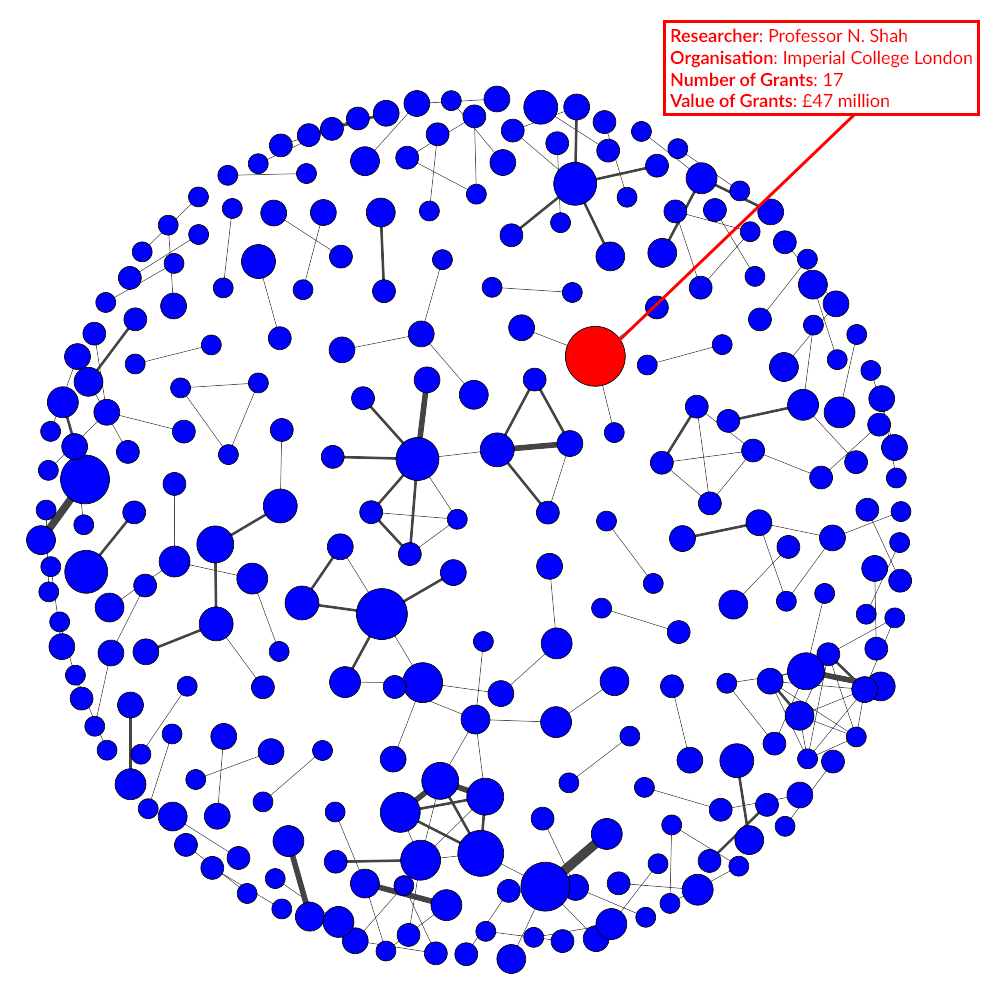
\includegraphics[width=8cm]{networks-explained/researcher_network_b}
    \caption[Visual explanation of how the \textit{Researcher-grant} network was structured and constructed using the collected EPSRC data]{Visual explanation of how the \textit{Researcher-grant} network was structured and constructed using the collected EPSRC data, including the formulated node and edge attributes.}
    \label{figure:researcher_b_structure}
\end{figure}

\subsection{Node and edge attributes}

The \textit{Researcher-grant} network contains two different node and edge attributes, the number and value of grants. Node and edge attributes are common between networks. Consequently, their formulation is considered a common task, and therefore it is described in Chapter \ref{chapter:methodology}: Methodology.

\subsection{Properties of Researcher-grant network}

The \textit{Researcher-grant} network is a carbon copy of the \textit{Topic-grant} network, with the exception that, in this case, nodes represent researchers and not topics. Table \ref{table:researcher_b_properties} presents the properties of both the historical and current \textit{Researcher-grant} networks.

\begin{table}[htbp]
\centering
\caption[Properties of the \textit{Researcher-grant} network constructed using both the historical (1990 to 2010) and current (2010 to 2016) data sets]{Properties of the \textit{Researcher-grant} network constructed using both the historical (1990 to 2010) and current (2010 to 2016) data sets.}
\label{table:researcher_b_properties}
\begin{tabular}{r|rrr}
{} & \textbf{1990-2000} & \textbf{2000-2010} & \textbf{2010-2016}\\
\hline\\
\textbf{Nodes}                          & {1847}   & {2434}    & {260}\\
\textbf{Edges}                          & {2002}   & {4919}    & {208}\\
\textbf{Type}                           & {Undirected} & {Undirected} & {Undirected}\\
\textbf{Weighted}                       & {Yes}    & {Yes}     & {Yes}\\
%\textbf{Connected}                     & {No}     & {No}      & {No}\\
\textbf{Average Degree}                 & {2.168}  & {4.042}   & {1.60}\\
\textbf{Average Weighted Degree}        & {2.798}  & {7.794}   & {2.592}\\
\textbf{Diameter}                       & {18.0}   & {36.0}    & {16.0}\\
%\textbf{Radius}                        & {1.0}    & {1.0}     & {1.0}\\
\textbf{Density}                        & {0.001}  & {0.002}   & {0.006}\\
\textbf{Modularity}                     & {0.978}  & {0.977}   & {0.955}\\
%\textbf{Communities}                   & {563}    & {485}     & {91}\\
%\textbf{Weak Components}                & {559}    & {473}     & {89}\\
%\textbf{Node Closeness}                & {0.001}  & {0.0}     & {0.004}\\
%\textbf{Node Betweenness}              & {14.214} & {138.711} & {1.965}\\
%\textbf{Edge Betweenness}              & {17.545} & {79.157}  & {4.625}\\
\textbf{Average Clustering Coefficient} & {0.648}  & {0.748}   & {0.578}\\
%\textbf{Eigenvector Centrality}        & {0.005}  & {0.007}   & {0.016}\\
\textbf{Average Path Length}            & {3.676}  & {6.874}   & {1.942}\\
\end{tabular}
\end{table}

The current \textit{Researcher-grant} network is composed of 260 nodes and 208 edges representing one or more common grants between two researchers. The network features a significantly disconnected structure, shown in Fig. \ref{figure:researcher_b_current_vis}, which is primarily due to the rarity in repeated collaboration among researchers on EPSRC-supported grants, which may last up to 8 years.

Furthermore, both historical \textit{Researcher-grant} networks consist of both an increased number of nodes and edges when compared to their current data equivalent. Furthermore, all three networks are weighted and in the in the creation of Table \ref{table:researcher_b_properties} and Fig. \ref{figure:researcher_b_current_vis}, the number of grants edge weight attribute is used.

\subsection{Visualisation of Researcher-grant network}

A visualisation of the \textit{Researcher-grant} network, presented in Fig. \ref{figure:researcher_b_current_vis}, was produced. It features nodes in blue, and edges in grey. The size of the node circle represents the number of grants node attribute. The width of the edge line represents the number of grants edge attribute. The researcher(s) that appear in the highest number of grant records are coloured in red.

\begin{figure}[htpb]
    \centering
    \fbox{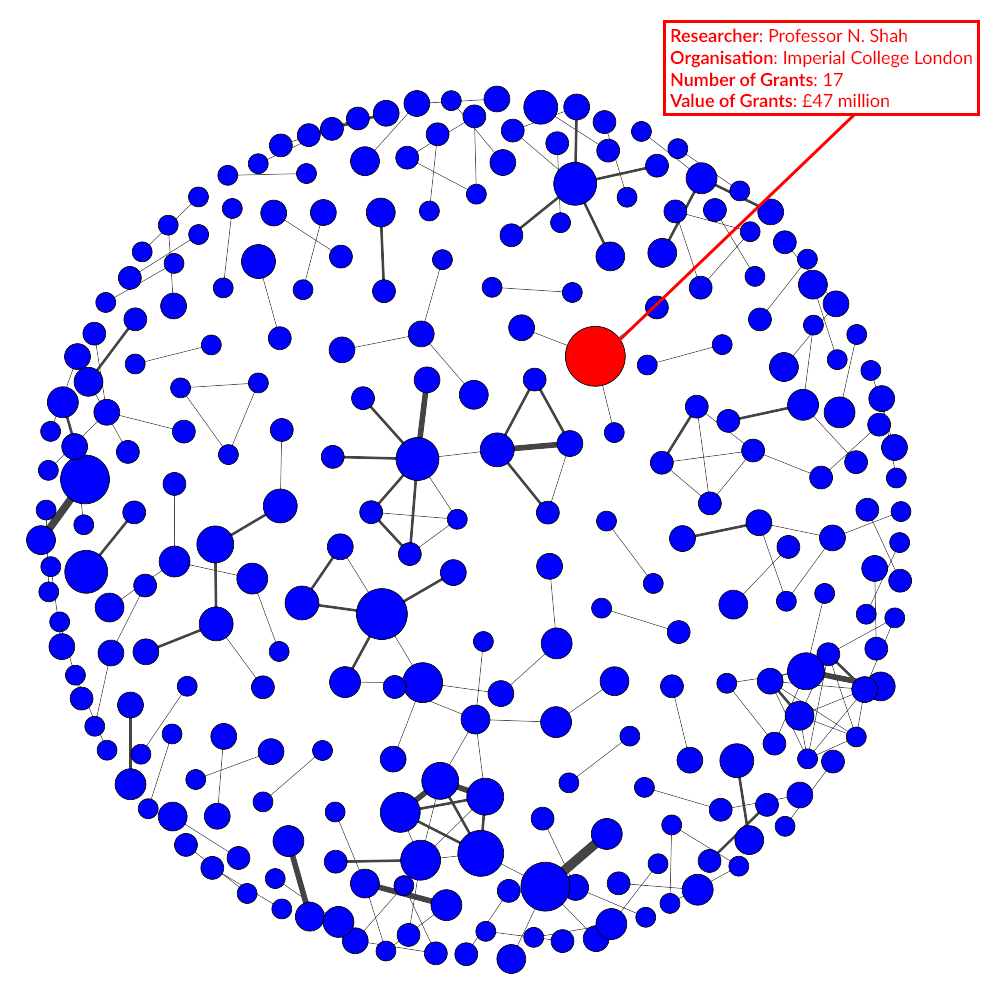
\includegraphics[width=12cm]{networks/researcher_b}}
    \caption[Visualisation of the \textit{Researcher-grant} network constructed using the current (2010 to 2016) data set.]{Visualisation of the \textit{Researcher-grant} network constructed using the current (2010 to 2016) data set. The researcher(s) that appear in the highest number of grant records are coloured in red.}
    \label{figure:researcher_b_current_vis}
\end{figure}

\section{Researcher-topic network}

The \textit{Researcher-topic} network consists of nodes representing researchers and edges representing topics. The \textit{Current EPSRC-Supported Research Topics} field in each researcher record consists of one or more topics that classify the grants supported by EPSRC that the researcher is currently an investigator in. Only researcher records with two or more topics were included in the analysis. Subsequently, each researcher record was compared to all other researcher records, and if they had at least one topic in common a link between the two researchers was established. The link signifies the topic(s) that two researchers have in common, and is represented as an edge in a network. Due to its significantly large size, the \textit{Researcher-topic} network was sampled and only includes nodes connected by edges with an edge weight of 5 or more. Fig. \ref{figure:researcher_a_structure} provides a visual explanation of how the \textit{Researcher-topic} network was constructed using the collected EPSRC data, including the formulated node and edge attributes.

\begin{figure}[htpb]
    \centering
    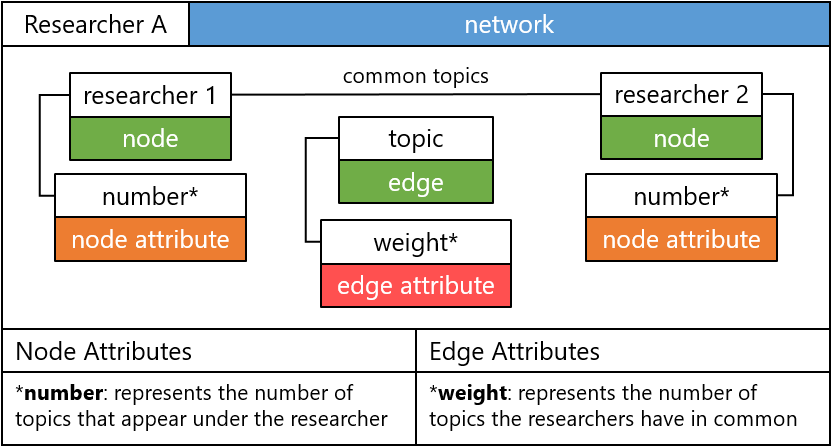
\includegraphics[width=8cm]{networks-explained/researcher_network_a}
    \caption[Visual explanation of how the \textit{Researcher-topic} network was structured and constructed using the collected EPSRC data]{Visual explanation of how the \textit{Researcher-topic} network was structured and constructed using the collected EPSRC data, including the formulated node and edge attributes.}
    \label{figure:researcher_a_structure}
\end{figure}

\subsection{Node and edge attributes}

The \textit{Researcher-topic} network contains one node and edge attribute, the number of topics. In the \textit{Researcher-topic network} edges represent topics, therefore, it does not contain the value of grants attribute. Node and edge attributes are common between networks. Consequently, their formulation is considered a common task, and therefore it is described in Chapter \ref{chapter:methodology}: Methodology.

\subsection{Properties of Researcher-topic network}

The \textit{Researcher-topic} network is a reversed version of the \textit{Topic-researcher} network. It consists of 655 researchers linked by 4548 edges representing common topics between the researchers. Table \ref{table:researcher_a_properties} presents the properties of the \textit{Researcher-topic} network.

\begin{table}[htbp]
\centering
\caption[Properties of the \textit{Researcher-topic} network constructed using the current (2010 to 2016) data set]{Properties of the \textit{Researcher-topic} network constructed using the current (2010 to 2016) data set.}
\label{table:researcher_a_properties}
\begin{tabular}{r|r}
{} & \textbf{2010-2016}\\
\hline\\
\textbf{Nodes}                          & {655}\\
\textbf{Edges}                          & {4548}\\
\textbf{Type}                           & {Undirected}\\
\textbf{Weighted}                       & {Yes}\\
%\textbf{Connected}                     & {No}\\
\textbf{Average Degree}                 & {13.887}\\
\textbf{Average Weighted Degree}        & {27.258}\\
\textbf{Diameter}                       & {15.0}\\
%\textbf{Radius}                        & {1.0}\\
\textbf{Density}                        & {0.021}\\
\textbf{Modularity}                     & {0.738}\\
%\textbf{Communities}                   & {49}\\
%\textbf{Weak Components}                & {39}\\
%\textbf{Node Closeness}                & {0.005}\\
%\textbf{Node Betweenness}              & {703.138}\\
%\textbf{Edge Betweenness}              & {127.386}\\
\textbf{Average Clustering Coefficient} & {0.825}\\
%\textbf{Eigenvector Centrality}        & {0.078}\\
\textbf{Average Path Length}            & {4.278}\\
\end{tabular}
\end{table}

In comparison to the current \textit{Researcher-grant} network which consists of 260 nodes and 208 edges, this network consists of substantially more nodes and edges. Due to its significantly large size, the \textit{Researcher-topic} network had to be sampled with the sample consisting of nodes connected by edges with an edge weight of 5 or more. Furthermore, the network is undirected and weighted and in the creation of Table \ref{table:researcher_a_properties} and Fig. \ref{figure:researcher_a_vis}, the number of topics edge weight attribute is used.

\subsection{Visualisation of the Research-topic network}

A visualisation of the \textit{Researcher-topic} network, presented in Fig. \ref{figure:researcher_a_vis}, was produced using iGraph. It features nodes in blue, and edges in grey. The size of the node circle represents the number of topics node attribute. The width of the edge line represents the number of topics edge attribute. The researcher(s) with the highest number of topics are coloured in red.

As illustrated in Fig. \ref{figure:researcher_a_vis}, the structure of the \textit{Researcher-topic} network stands out from the others. Both \textit{Topic} networks feature a conglomeration of nodes densely connected. In contrast, the \textit{Researcher-grant} network consists the opposite of that, as it is sparsely connected with up to a maximum of 4 connected nodes. The \textit{Researcher-topic} network represents a combination between the two. Based on an initial observation, an unsurprising guess would indicate that a community detection algorithm has already been applied to this network. However, it has not, as its structure clearly resembles the layout of collaboration between researchers. Several small groups of researchers, densely connected internally, but sparsely connected externally, can be spotted. This can also translate to the assumption that the communities represent common topic interests between researchers.

\begin{figure}[htpb]
    \centering
    \fbox{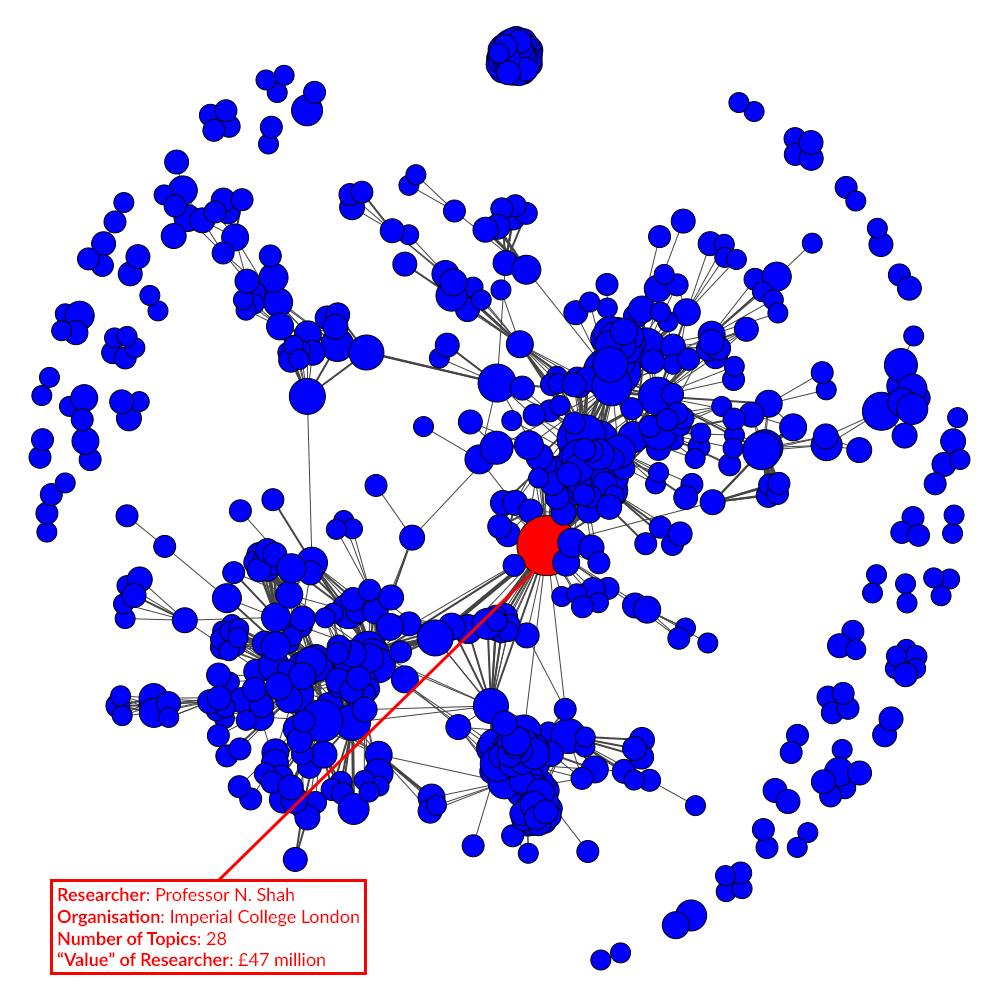
\includegraphics[width=11.5cm]{networks/researcher_a}}
    \caption[Visualisation of the \textit{Researcher-topic} network constructed using the current (2010 to 2016) data set]{Visualisation of the \textit{Researcher-topic} network constructed using the current (2010 to 2016) data set. The researcher(s) with the highest number of topics are coloured in red.}
    \label{figure:researcher_a_vis}
\end{figure}